\documentclass{beamer}
\usetheme{metropolis}
\usepackage{graphicx}
\usepackage{tabularx}
\usepackage{hyperref}

\title{Benefits of Open Science for Students}
\author{\parbox{\textwidth}{Konsta Happonen\\
    Open Knowledge Finland - Open Science Working Group\\
    \\
    \href{http://twitter.com/koalha}{@Koalha}\\
    \url{http://github.com/koalha/oaweek2016}}\\
}
\date{}
\usebackgroundtemplate{
\includegraphics{light-grey-rgb.pdf}}

\begin{document}
\maketitle


\begin{frame}{What is Openness in the context of research and higher education?}

  \begin{quote}
    Open science is the movement to make scientific research, data and dissemination accessible to all levels of an inquiring society, amateur or professional.\\
    \flushright {\normalfont Wikipedia article on Open Science}
  \end{quote}

\end{frame}

\begin{frame}{Why is Openness important for students?}

  Higher education often hampered by hassle with licences and copyright.

  Lecture materials and articles are often distributed illegally or as useless versions stripped of copyrighted material.

  Textbooks are in short-supply and/or contain outdated information.

  University provides for its students, but what about after graduation?

\end{frame}

\begin{frame}{What types of Open are there?}
  \begin{enumerate}
  \item Open Educational Resources
  \item Open Access to Literature
  \item Free Software
  \end{enumerate}
\end{frame}

\begin{frame}{Open Educational Resources}
  \begin{center}
    
\includegraphics[height=0.6\textheight]{wikibooks.png}
  \end{center}
  
  Textbooks cost money
  
  Copyright laws make distributing educational materials (such as lecture slides) illegal

  \tiny{image source: \href{https://upload.wikimedia.org/wikipedia/commons/thumb/7/7c/Wikibooks-logo-en.svg/600px-Wikibooks-logo-en.svg.png}{Bastique / Wikipedia}}
\end{frame}

\begin{frame}{Open Access to Literature}
  \begin{center}
    
\includegraphics[height = 0.6\textheight]{oalogo.png}
  \end{center}

  Access to literature may be hindered after graduating\\
  Rising subscription costs mean teachers and students don't have access to all key literature
\end{frame}

\begin{frame}{Free software}
  \begin{center}
    
\includegraphics[height=0.4\textheight]{tux.png}
  \end{center}
  
  Use of proprietary software often doesn't allow training at home.
  
  Many software providers offer affordable student licences, but graduating might mean being reliant on software whose licences cost hundreds or thousands of dollars.

  Even then universities have to pay for the licences, and the money is away from something else.
\end{frame}

\begin{frame}{Free software - example}
  \begin{tabularx}{\textwidth}{lXl}
     & \textbf{ESRI ArcGIS} & \textbf{QGIS}\\
    Student licence & free to use via VPN & Free\\
    Licence for personal use & 100 \$ / year & Free\\
    Licence for commercial use & 1500 \$ / year & Free
  \end{tabularx}
\end{frame}

\begin{frame}{Licence fees keep growing at a ~10\%/year rate...}
  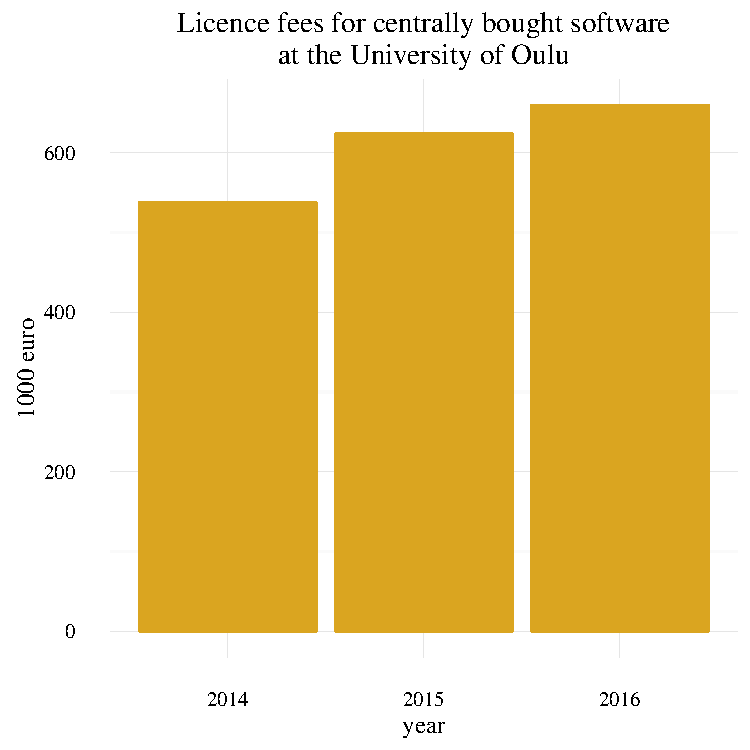
\includegraphics[width=0.5\textwidth]{licencefees.pdf}
  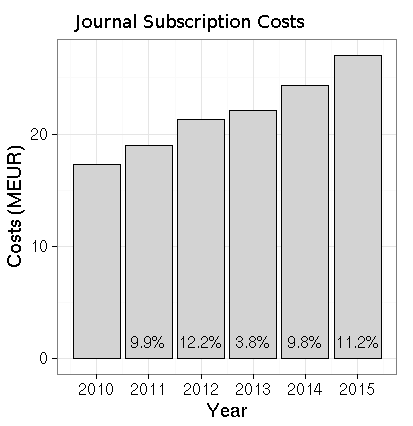
\includegraphics[width=0.5\textwidth]{subscriptioncosts.png}

  \tiny{sources: University of Oulu IT administration \& \url{http://ropengov.github.io/r/2016/06/10/FOI/}}
\end{frame}

\begin{frame}{...at the same time, universities suffer funding cuts}
  \begin{center}
    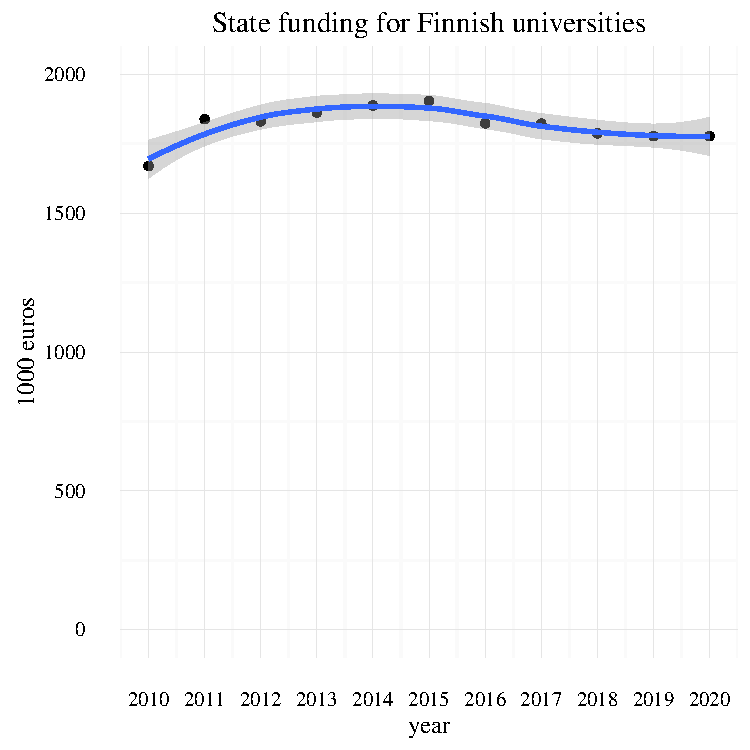
\includegraphics[height=0.8\textheight]{unifund.pdf}
  \end{center}
  
  \tiny{source: \url{https://twitter.com/KuuttiUusitalo/status/709097070343356416}}
\end{frame}

\begin{frame}{Interested in openness?}
  Join Open Knowledge Finland, it's free: \url{http://fi.okfn.org/membership/}
  
  Open Science Working Group on facebook: \url{https://www.facebook.com/groups/open.science.fi/}
\end{frame}

\end{document}
